\chapter{Parallel Management of Topological Transitions}
%\section{Parallel Management of Topological Transitions}
\label{chap:parallelflip}

\lettrine{A}{s} discussed in Chapter \ref{chap:2dgrains}, topological transitions modify the grain structure and data structure must reflect this relations at every time step. The update of this structure is critical, due to the consistency during numerical simulation and implementation performance. We discuss here the sequential management algorithm of topological transitions in a grain growth numerical simulation and then we propose a parallel management algorithm that aims to handle a great number of grains.

\section{Sequential Management}

The Coupled Model and Stored Energy Model developed in Chapter \ref{chap:coupledmodel} and \ref{chap:storedenergy} both relies on the linked data structure of vertices linked to three grain boundaries, and grain boundaries linked to two vertices. In a sequential implementation of these models the transitions can be detected by estimating the time that a boundary will collapse, named extinction time or $t_{\text{ext}}$. If the extinction time lies in the current time step $[t, t + \Delta t]$, the boundary is considered to flip and we say this boundary is a candidate. A simple algorithm to solve the transitions within the time step is to sort the candidate boundaries by their extinction time in decreasing order. We can iteratively solve the conflicts by labeling those candidates involved in transitions of other candidates, the labeled boundaries are inhibited to flip this time step. Once all the conflicts has been solved the transitions are performed. Algorithm \ref{alg:seqtopological} summarizes the described management.

\begin{algorithm}
\caption{Sequential Management of Topological Transitions}
\label{alg:seqtopological}
\begin{algorithmic}[1]
\Procedure{Sequential}{}
\State $\boundaries \gets$ Clear flip and inhibited state for each boundary
\State $\boundaries \gets$ Update $t_{\text{ext}}$ for each boundary
\State $\boundaries_{\text{flip}} \gets$ Boundaries to flip with $t_{\text{ext}} \in [0, \Delta t]$ 
\State $\boundaries_{\text{flip}} \gets$ Sort boundaries by $t_{\text{ext}}$ in decreasing order
\State $\boundaries_{\text{tmp}} \gets \varnothing,\quad$ Empty list of boundaries visited
\State $\vertices_{\text{tmp}} \gets \varnothing,\quad$ Empty list of vertices visited
\ForEach{$\Gamma \in \boundaries_{\text{flip}}$}
    \State $\{\x_i, \x_j\} \gets $ Vertices of $\Gamma$
    \If{$ \vertices_{\text{tmp}} \cap \{\x_i, \x_j\} = \varnothing$}
        \State $\boundaries_{\text{tmp}} \gets \boundaries_{\text{tmp}} \cup \Gamma$
        \State $\vertices_{\text{tmp}} \gets \vertices_{\text{tmp}} \cup \{\x_i, \x_j\}$
    \Else
        \State \Return $\boundaries_{\text{tmp}}$
    \EndIf
    %\State $\boundaries_{\text{I}} \gets$ Set of neighbor boundaries to $\Gamma$
    %\State $\boundaries_{\text{flip}} \gets \boundaries_{\text{flip}} \setminus \boundaries_{\text{I}}$ Inhibit boundaries to flip
\EndFor
\EndProcedure
\end{algorithmic}
\end{algorithm}

Due to the need of more significant statistics, hundreds of thousands of grains must be simulated. A sequential approach might be inefficient, and parallel implementation of the presented models is proposed. The parallel implementation is straightforward when we speak of evolving the data structure, but the problem of solve the topological transitions arise since the mechanism to solve inconsistencies is sequential and parallelism over data structure will generate race conditions.

\section{Parallel Polling System}

Since the concurrent access to data structure in a parallel implementation makes the sequential approach of managing topological transitions a bottleneck, a management system is proposed based on local information given by vertices and boundaries. First we need to compute the extinction time for each boundary and label the candidates for flipping. Instead of sorting the boundaries as the sequential algorithm, each vertex will store local information on which boundary has the lowest extinction time. We say that each vertex \emph{voted} for a boundary. Next, each boundary counts the obtained votes by referring to its vertices. The vote counting is meaningful, two votes means that a boundary can flip since all their neighbor boundaries have not collided yet, and earns the right to label neighbor boundaries to not flip this time step. Other boundaries will obtain one or zero votes.
This polling is repeated until no further labeling is possible, that is, when the previous set of candidates is the same as the next iteration.

Figure \ref{fig:pollingscheme} shows a brief example of the polling system. Consider a neighborhood of boundaries with their extinction times already computed. Figure \ref{fig:poll1} shows the vertex poll. Each vertex in this neighborhood will vote for their boundary with lowest $t_{\text{ext}}$. We can see that some boundaries obtained zero, one or two votes. The case of a boundary with two votes is special because implies that two vertices (pink and green) decided that their shared boundary is a good candidate and therefore no other boundary in the immediate neighborhood is a flipping candidate where they obtained at most one vote. Figure \ref{fig:poll2} shows the final counting for each boundary. Boundaries with zero votes remain in black, boundaries with one votes are cyan and boundaries with two votes are red. Notice that although cyan boundaries might be able to flip, the priority is assigned to boundaries with two votes and they label their neighbor boundaries as inhibited as shown in Figure \ref{fig:poll3}. Inhibited boundaries, in gray, can't be voted at next iteration. Related vertices must vote between the remaining non-inhibited boundaries, as shown in Figure \ref{fig:poll4}.

\begin{figure}[t]
    \centering
    \subfloat[] {    
    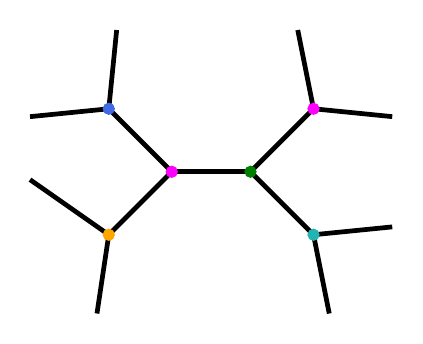
\begin{tikzpicture}
    % Boundaries
    \draw[line width=0.6mm, black] (0,0) -- (1,0);
    %
    \draw[line width=0.6mm, black] (0,0) -- (-0.8,0.8);
    \draw[line width=0.6mm, black] (-0.8,0.8) -- (-0.7, 1.8);
    \draw[line width=0.6mm, black] (-0.8,0.8) -- (-1.8,0.7);
    %
    \draw[line width=0.6mm, black] (0,0) -- (-0.8,-0.8);
    \draw[line width=0.6mm, black] (-0.8,-0.8) -- (-1.8, -0.1);
    \draw[line width=0.6mm, black] (-0.8,-0.8) -- (-0.95, -1.8);
    %
    \draw[line width=0.6mm, black] (1,0) -- (1.8,0.8);
    \draw[line width=0.6mm, black] (1.8,0.8) -- (1.6, 1.8);
    \draw[line width=0.6mm, black] (1.8,0.8) -- (2.8,0.7);
    %
    \draw[line width=0.6mm, black] (1,0) -- (1.8,-0.8);
    \draw[line width=0.6mm, black] (1.8,-0.8) -- (2, -1.8);
    \draw[line width=0.6mm, black] (1.8,-0.8) -- (2.8,-0.7);
    % Vertices
    \filldraw [Magenta] (0,0) circle (2pt);
    \filldraw [RoyalBlue] (-0.8,0.8) circle (2pt);
    \filldraw [Orange] (-0.8,-0.8) circle (2pt);
    \filldraw [Green] (1,0) circle (2pt);
    \filldraw [Fuchsia] (1.8,0.8) circle (2pt);
    \filldraw [TealBlue] (1.8,-0.8) circle (2pt);
    % Votes
    \node[draw=none, color=Magenta] at (0.5, -0.3) {$\checkmark$};
    \node[draw=none, color=RoyalBlue] at (-0.5, 1.2) {$\checkmark$};
    \node[draw=none, color=Orange] at (-0.3, -0.6) {$\checkmark$};
    \node[draw=none, color=Green] at (0.5, 0.3) {$\checkmark$};
    \node[draw=none, color=Fuchsia] at (1.3, 0.6) {$\checkmark$};
    \node[draw=none, color=TealBlue] at (2.3, -0.45) {$\checkmark$};
    %%
    \end{tikzpicture}
    \label{fig:poll1}
    }\hspace{5em}
    \subfloat[] {    
    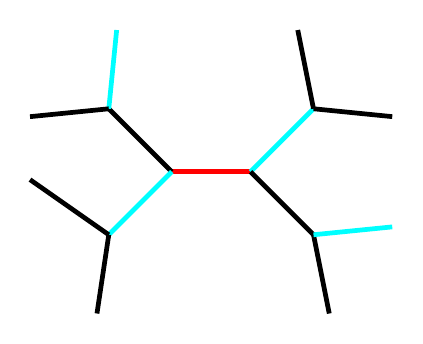
\begin{tikzpicture}
    % Boundaries
    \draw[line width=0.6mm, red] (0,0) -- (1,0);
    %
    \draw[line width=0.6mm, black] (0,0) -- (-0.8,0.8);
    \draw[line width=0.6mm, Cyan] (-0.8,0.8) -- (-0.7, 1.8);
    \draw[line width=0.6mm, black] (-0.8,0.8) -- (-1.8,0.7);
    %
    \draw[line width=0.6mm, Cyan] (0,0) -- (-0.8,-0.8);
    \draw[line width=0.6mm, black] (-0.8,-0.8) -- (-1.8, -0.1);
    \draw[line width=0.6mm, black] (-0.8,-0.8) -- (-0.95, -1.8);
    %
    \draw[line width=0.6mm, Cyan] (1,0) -- (1.8,0.8);
    \draw[line width=0.6mm, black] (1.8,0.8) -- (1.6, 1.8);
    \draw[line width=0.6mm, black] (1.8,0.8) -- (2.8,0.7);
    %
    \draw[line width=0.6mm, black] (1,0) -- (1.8,-0.8);
    \draw[line width=0.6mm, black] (1.8,-0.8) -- (2, -1.8);
    \draw[line width=0.6mm, Cyan] (1.8,-0.8) -- (2.8,-0.7);
    \end{tikzpicture}
    \label{fig:poll2}
    }
    \\
    \subfloat[] {    
    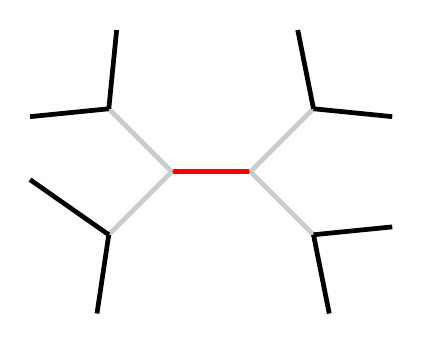
\begin{tikzpicture}
    % Boundaries
    \draw[line width=0.6mm, red] (0,0) -- (1,0);
    %
    \draw[line width=0.6mm, black!20] (0,0) -- (-0.8,0.8);
    \draw[line width=0.6mm, black] (-0.8,0.8) -- (-0.7, 1.8);
    \draw[line width=0.6mm, black] (-0.8,0.8) -- (-1.8,0.7);
    %
    \draw[line width=0.6mm, black!20] (0,0) -- (-0.8,-0.8);
    \draw[line width=0.6mm, black] (-0.8,-0.8) -- (-1.8, -0.1);
    \draw[line width=0.6mm, black] (-0.8,-0.8) -- (-0.95, -1.8);
    %
    \draw[line width=0.6mm, black!20] (1,0) -- (1.8,0.8);
    \draw[line width=0.6mm, black] (1.8,0.8) -- (1.6, 1.8);
    \draw[line width=0.6mm, black] (1.8,0.8) -- (2.8,0.7);
    %
    \draw[line width=0.6mm, black!20] (1,0) -- (1.8,-0.8);
    \draw[line width=0.6mm, black] (1.8,-0.8) -- (2, -1.8);
    \draw[line width=0.6mm, black] (1.8,-0.8) -- (2.8,-0.7);
    \end{tikzpicture}
    \label{fig:poll3}
    }\hspace{5em}
    \subfloat[] {    
    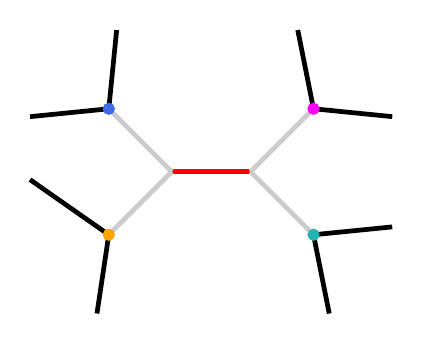
\begin{tikzpicture}
    % Boundaries
    \draw[line width=0.6mm, red] (0,0) -- (1,0);
    %
    \draw[line width=0.6mm, black!20] (0,0) -- (-0.8,0.8);
    \draw[line width=0.6mm, black] (-0.8,0.8) -- (-0.7, 1.8);
    \draw[line width=0.6mm, black] (-0.8,0.8) -- (-1.8,0.7);
    %
    \draw[line width=0.6mm, black!20] (0,0) -- (-0.8,-0.8);
    \draw[line width=0.6mm, black] (-0.8,-0.8) -- (-1.8, -0.1);
    \draw[line width=0.6mm, black] (-0.8,-0.8) -- (-0.95, -1.8);
    %
    \draw[line width=0.6mm, black!20] (1,0) -- (1.8,0.8);
    \draw[line width=0.6mm, black] (1.8,0.8) -- (1.6, 1.8);
    \draw[line width=0.6mm, black] (1.8,0.8) -- (2.8,0.7);
    %
    \draw[line width=0.6mm, black!20] (1,0) -- (1.8,-0.8);
    \draw[line width=0.6mm, black] (1.8,-0.8) -- (2, -1.8);
    \draw[line width=0.6mm, black] (1.8,-0.8) -- (2.8,-0.7);
    % Vertices
    %\filldraw [Magenta] (0,0) circle (2pt);
    \filldraw [RoyalBlue] (-0.8,0.8) circle (2pt);
    \filldraw [Orange] (-0.8,-0.8) circle (2pt);
    %\filldraw [Green] (1,0) circle (2pt);
    \filldraw [Fuchsia] (1.8,0.8) circle (2pt);
    \filldraw [TealBlue] (1.8,-0.8) circle (2pt);
    % Votes
    \node[draw=none, color=RoyalBlue] at (-0.5, 1.2) {$\checkmark$};
    \node[draw=none, color=Orange] at (-1.4, -0.7) {$\checkmark$};
    \node[draw=none, color=Fuchsia] at (2, 1.6) {$\checkmark$};
    \node[draw=none, color=TealBlue] at (2.3, -0.45) {$\checkmark$};
    \end{tikzpicture}
    \label{fig:poll4}
    }
    \caption{Polling system scheme.}
    \label{fig:pollingscheme}
\end{figure}


This procedure can be seen as a fixed point iteration over a polling function $\text{Poll}(\mathcal{S})$, where the input of the system $\mathcal{S}$ is the inhibited state of each boundary. When the polling function, given an inhibited state, returns the same inhibited state, we have found a fixed point of the function and thus we converged to a feasible solution. Algorithm \ref{alg:polling} summarizes this idea.
\begin{algorithm}
\caption{Polling Routine for Inhibit Boundaries}
\label{alg:pollroutine}
\begin{algorithmic}[1]
\Procedure{Poll}{$\mathcal{S}$}
\State $\boundaries_{\text{flip}} \gets$ Clear boundaries count to 0 and vertices votes
\State $\boundaries_{\text{flip}} \gets$ Vertices votes for their uninhibited boundary with lowest $t_{\text{ext}}$
\State $\boundaries_{\text{flip}} \gets$ Boundaries counts the votes received
\State $\boundaries_{\text{flip}} \gets$ Select uninhibited boundaries with two votes
\State $\boundaries_{\text{flip}} \gets$ Inhibit neighbor boundaries
\State \Return $\mathcal{S}$ \Comment{New inhibited state of boundaries}
\EndProcedure
\end{algorithmic}
\end{algorithm}

\begin{algorithm}
\caption{Parallel Polling System for Managing Topological Transitions}
\label{alg:polling}
\begin{algorithmic}[1]
\Procedure{Polling\_System}{}
\State $\boundaries \gets$ Clear flip and inhibited state for each boundary
\State $\boundaries \gets$ Update $t_{\text{ext}}$ for each boundary
\State $\boundaries_{\text{flip}} \gets$ Boundaries to flip with $t_{\text{ext}} \in [0, \Delta t]$
\State $\mathcal{S}_0 \gets$ Initial inhibited state of boundaries
%\State $convergence \gets$ False
\For {$i: 1,\dotsc,n$}
    \State $\mathcal{S}_i \gets \textsc{Poll}(\mathcal{S}_{i-1})$
    \If{$\mathcal{S}_i = \mathcal{S}_{i-1}$}
    \State \Return
    \EndIf
%\While {$!convergence$}
%\State $I_{\text{prev}} \gets $ Inhibited state of boundaries.
%\State $\Gamma_{\text{flip}} \gets$ Clear boundaries count to 0 and vertices votes
%\State $\Gamma_{\text{flip}} \gets$ Vertices votes for their uninhibited boundary with lowest $t_{ext}$
%\State $\Gamma_{\text{flip}} \gets$ Boundaries counts the votes received
%\State $\Gamma_{\text{flip}} \gets$ Select uninhibited boundaries  with two votes and inhibit neighbor boundaries
%\State $I \gets$ New inhibited state of boundaries
%\If{$I \setminus I_{\text{prev}} =  \varnothing$}
%\State $convergence \gets$ True
%\EndIf
%\EndWhile
\EndFor
\EndProcedure
\end{algorithmic}
\end{algorithm}

The advantage of this system is that the vertices votes and boundaries counting can be performed in parallel since data is accessed as read-only. No race condition exists here since we avoided possible near flippings. One disadvantage is the computational cost of perform the polling iteratively until convergence, but the number of topological transitions over time tend to decrease, thus this algorithm is in practice fast enough.
%Parallel implementation of these models is straightforward without taking in account the transitions, but once we reach the critical time that these transitions occur, it is possible that concurrent access to vertices and boundaries data structure generate race conditions.
